\section{Pesudocode of \ourmethod}


To improve the clarity, we provide additional details regarding the regression model fitting process and the data used. Specifically, the regression model is trained using $N$ data points generated by evaluating proxy models on randomly sampled data mixtures. 
A pseudocode representation of the Algorithm~\ref{alg:regmix} is included below to outline the procedure.

\begin{algorithm}[htbp]
\caption{\ourmethod: Data Mixture as Regression}
\label{alg:regmix}
\begin{algorithmic}[1]
\STATE \textbf{Input:} Token mixtures for $n$ domains $\mathbf{x}^0 = \{x_1^0, x_2^0, \dots, x_n^0\}$, number of proxy models $N$, target metric $y$, and regression model $f$
\STATE \textbf{Output:} Optimal data mixture $\mathbf{x}^* = \{x_1^*, x_2^*, \dots, x_n^*\}$

\STATE \textbf{Step 1: Train Proxy Models}
\STATE Generate $N$ random data mixtures $\{\mathbf{x}_i\}_{i=1}^N$, where each $\mathbf{x}_i = \{x_1^i, x_2^i, \dots, x_n^i\}$ is sampled from a Dirichlet distribution $\text{Dir}(\mathbf{\alpha} = \lambda \cdot \mathbf{x}^0)$, with $\lambda \in [0.1, 5.0]$ to ensure diversity.
\FOR{each mixture $\mathbf{x}_i$}
    \STATE Train a small-scale proxy model using $\mathbf{x}_i$ for a fixed number of tokens.
    \STATE Evaluate the proxy model to compute the target metric $y_i$ (e.g., validation loss).
\ENDFOR

\STATE \textbf{Step 2: Fit Regression Model}
\STATE Use $\{(\mathbf{x}_i, y_i)\}_{i=1}^N$ to train the regression model $f(\mathbf{x})$ to predict $y$.

\STATE \textbf{Step 3: Simulate Data Mixtures and Predict Performance}
\STATE Generate a large set of candidate mixtures $\{\mathbf{x}_j\}_{j=1}^M$.
\STATE Predict the target metric for each mixture: $y_j = f(\mathbf{x}_j)$.
\STATE Identify the mixture $\mathbf{x}^*$ that minimizes $y$: $\mathbf{x}^* = \arg\min_{\mathbf{x}_j} f(\mathbf{x}_j)$.

\STATE \textbf{Step 4: Train Large-Scale Model}
\STATE Use the identified optimal mixture $\mathbf{x}^*$ to train a large-scale model with significantly more tokens. Optionally, average top-performing mixtures for robustness.

\STATE \textbf{Return:} Optimal data mixture $\mathbf{x}^*$
\end{algorithmic}
\end{algorithm}


\clearpage

\section{Rank Invariance Hypothesis}

The rank invariance hypothesis asserts that the relative rankings of data mixtures should remain stable across varying model sizes (e.g., from 1M to 1B parameters) and token scales (e.g., from 1B to 25B tokens). 
This hypothesis suggests that the comparative effectiveness of different data mixtures does not significantly change as models grow in size or are trained on larger amounts of tokens.

To examine this hypothesis, we conducted a comprehensive set of experiments involving models of four distinct scales: 1M, 60M, 280M, and 1B parameters. 
Each model was trained using 64 different data mixture configurations, where the token amounts varied systematically. 
For each setting, we measured the validation loss for all data mixtures and determined their rankings. 
To quantify the consistency of rankings across model sizes and token scales, we computed the Spearman rank correlation coefficient ($\rho$) for each comparison.

The results shown in Figure~\ref{fig:corr_heatmap}, reveal high rank correlation coefficients across all model and token scales. 
This finding provides strong empirical support for the rank invariance hypothesis, indicating that the relative utility of data mixtures is robust to changes in model size and training tokens.

\begin{figure}[htbp]
    \centering
    \subfigure{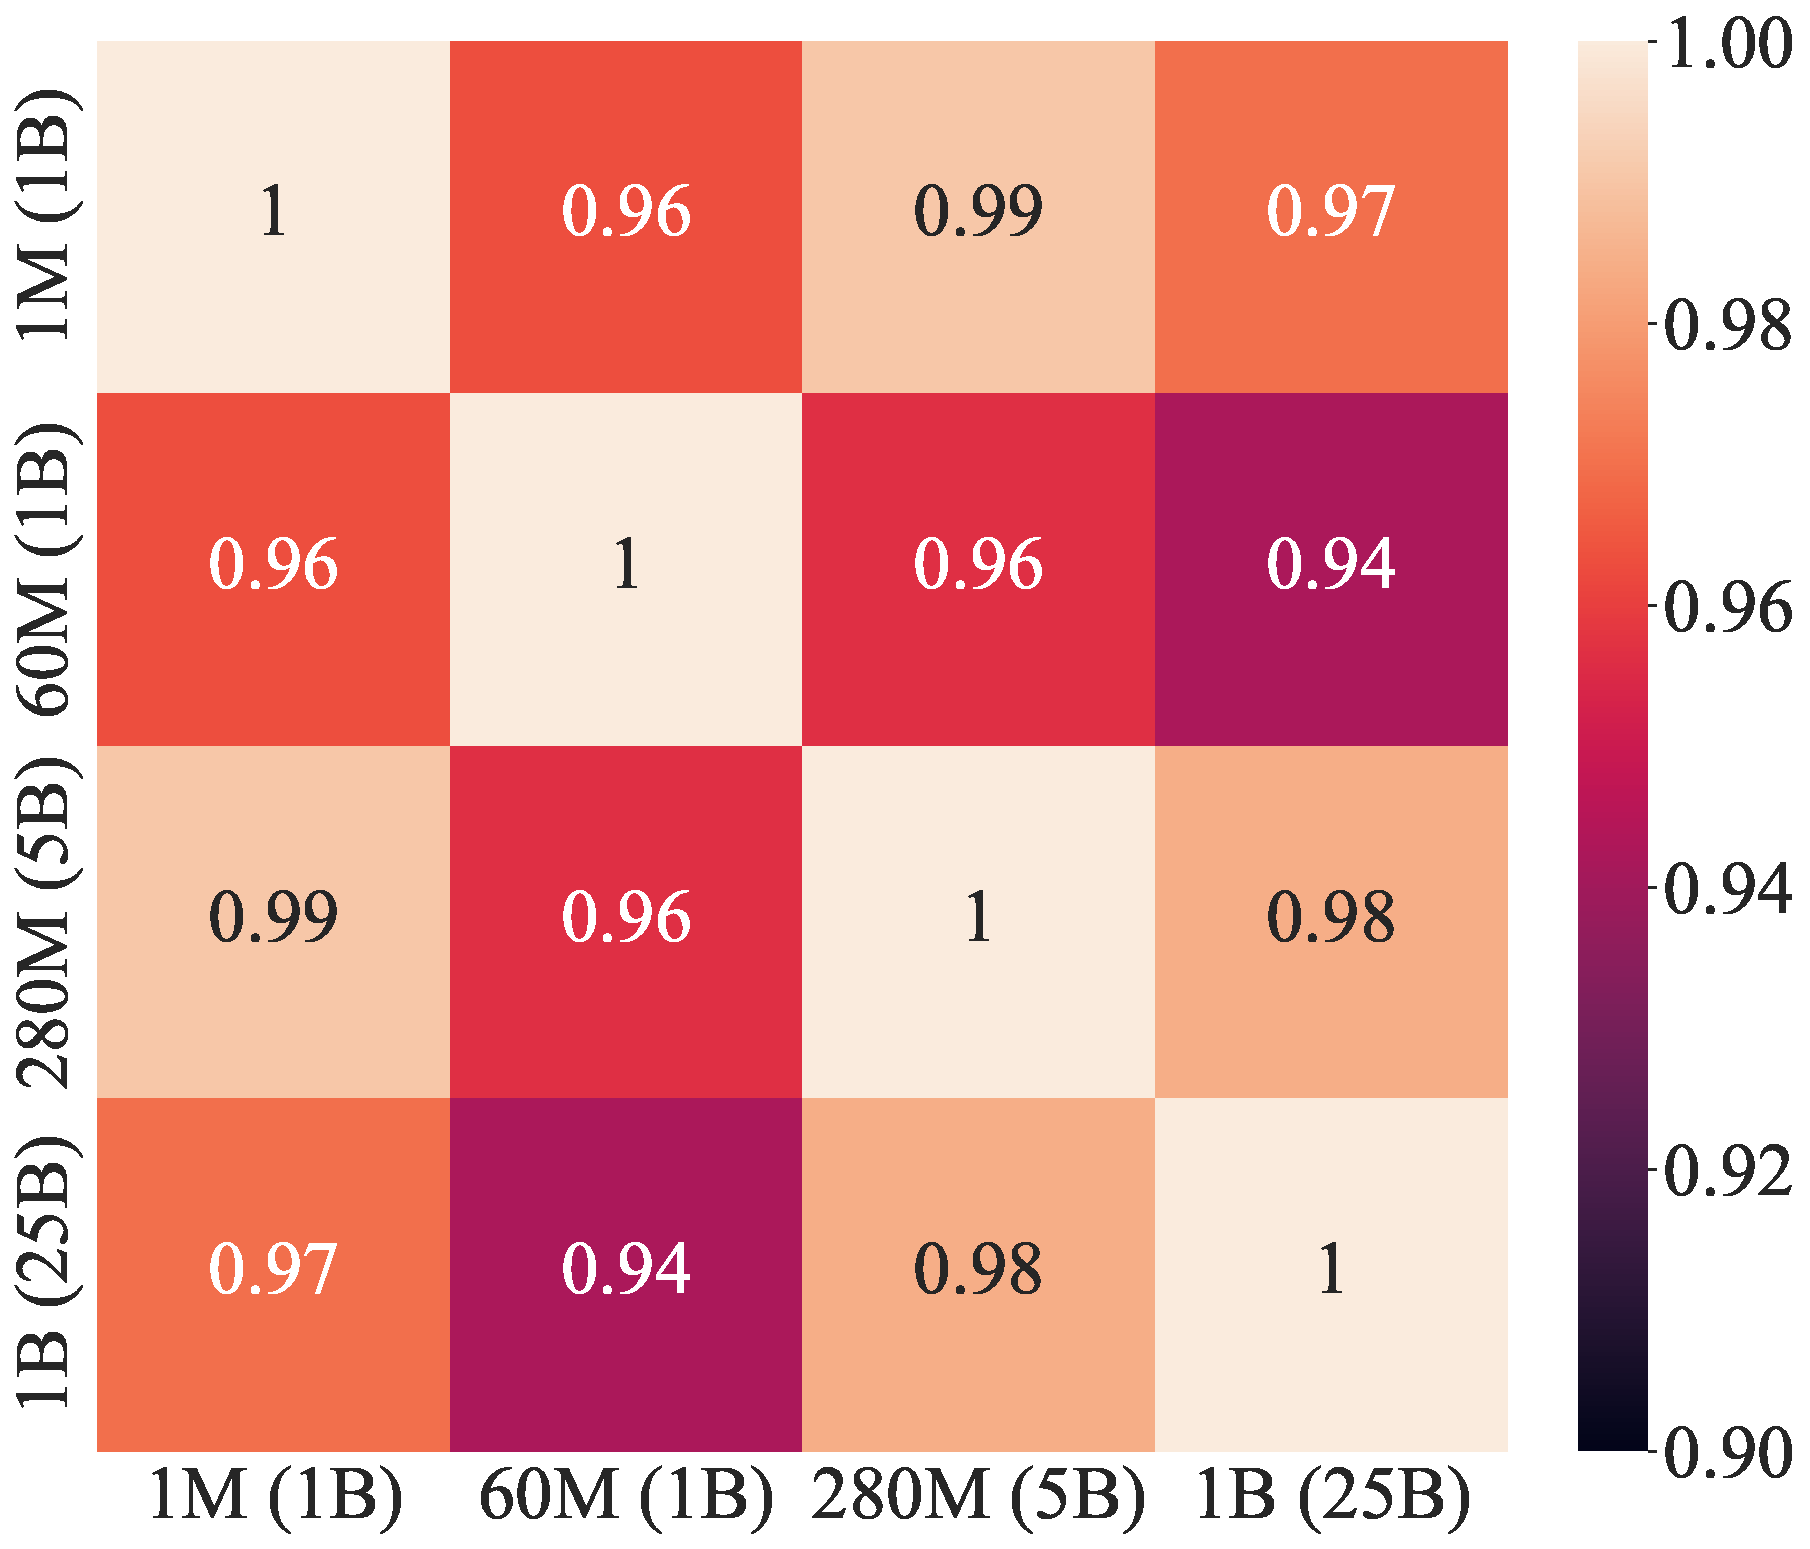
\includegraphics[width=0.45\textwidth]{figures/rebuttal/corr_heatmap.pdf}}
    \caption{ Heatmap of Spearman rank correlation coefficients ($\rho$) between validation loss rankings for different model scales (1M, 60M, 280M, and 1B parameters) and token scales (1B, 10B, and 25B tokens). The consistently high correlation values across all settings support the rank invariance hypothesis, indicating that the relative ranking of data mixtures remains stable despite changes in model size and training scale.}
    \label{fig:corr_heatmap}
\end{figure}


\begin{table}[b]
    \centering
    \small
    \label{tab:regmix_human_7b}
    \caption{Performance comparison between Human and RegMix on 7B models trained on 100B tokens across 13 downstream benchmarks.}
    \begin{tabular}{ccc}
    \toprule
    \textbf{Benchmark} & \textbf{Human} & \textbf{\ourmethod} \\
    \midrule
         Social IQA & 41.6 & 43.3 \\
         HellaSwag & 55.0 & 63.3 \\
         PiQA & 72.4 & 75.3 \\
         OpenBookQA & 34.1 & 36.7 \\
         Lambada & 44.9 & 51.0 \\
         SciQ & 91.7 & 91.2 \\
         ARC Easy & 63.5 & 65.4\\
         COPA & 75.0 & 80.1\\
         RACE & 35.1 & 36.6 \\
         LogiQA & 25.7 & 24.1 \\
         QQP & 58.9 & 56.1 \\
         WinoGrande & 58.6 & 60.7 \\
         MultiRC & 52.6 & 51.0 \\
         \midrule
         Average & 54.5 & 56.5 (+2.0) \\
        \bottomrule
    \end{tabular}
\end{table}

\section{Scaling \ourmethod to 7B Models over 100B Tokens}

To further validate the effectiveness of our method on larger models, we conducted an experiment using Human baseline and our method data mixtures on a 7B model trained on 100B tokens. The results, summarized in Table~\ref{tab:regmix_human_7b}, demonstrate that RegMix still outperforms the Human baseline, achieving an average performance boost of 2\%.

To provide a closer illustration, we benchmark the downstream performance of RegMix and Human on every dataset at intervals of 25B tokens in Figure~\ref{fig:regmix_human_7b}. The results show that RegMix can significantly speed up pre-training, with a 50\% acceleration on most benchmarks (e.g., HellaSwag) and up to 75\% on some benchmarks (e.g., PiQA). Notably, the performance boost does not decrease with the amount of training tokens. However, we also observed that RegMix and Human struggle to improve on certain benchmarks (e.g., MultiRC), even with increased token amounts.
These findings suggest that RegMix can almost benefit downstream tasks whose performance increases with the amount of training data, but may not improve tasks that do not follow scaling laws. This observation is quite intriguing and warrants further investigation.

\section{Using Larger Proxy Model}

We conducted a preliminary study on the impact of proxy model size on effectiveness. Specifically, we compared two configurations: (1) 128 proxy models of 1B parameters each, and (2) 512 proxy models of 1M parameters each (the setting used in our main experiments). Both configurations used 1B training tokens per proxy model. We limited our investigation to these configurations due to computational constraints that prevented us from exploring scenarios with more 1B-parameter proxy models.

\begin{table}[htbp]
    \centering
    \label{tab:regmix_1m_1b}
    \caption{Performance comparison of optimized data mixtures derived from two proxy configurations (512$\times$ 1M and 128$\times$ 1B) for 7B models trained on 100B tokens, evaluated across 13 downstream benchmarks.}
    \begin{tabular}{ccc}
    \toprule
    \textbf{Benchmark} & \textbf{\ourmethod} (1B as proxy) & \textbf{\ourmethod} (1M as proxy) \\
    \midrule
         Social IQA & 43.4 & 43.3 \\
         HellaSwag & 62.9 & 63.3 \\
         PiQA & 75.1 & 75.3 \\
         OpenBookQA & 36.2 & 36.7 \\
         Lambada & 50.0 & 51.0 \\
         SciQ & 91.2 & 91.2 \\
         ARC Easy & 65.9 & 65.4\\
         COPA & 79.6 & 80.1\\
         RACE & 35.6 & 36.6 \\
         LogiQA & 23.9 & 24.1 \\
         QQP & 56.6 & 56.1 \\
         WinoGrande & 60.7 & 60.7 \\
         MultiRC & 51.6 & 51.0 \\
         \midrule
         Average & 56.4 & 56.5 \\
        \bottomrule
    \end{tabular}
\end{table}

To evaluate these configurations, we used their respective optimized data mixtures to train two 7B models on 100B tokens and compared their performance. The results, summarized in Table~\ref{tab:regmix_1m_1b}, show that both proxy settings achieved similar average performance across downstream tasks. This suggests that increasing proxy model size, even with fewer proxy models, can maintain competitive performance. However, given that the 1B proxy models do not significantly outperform the 1M proxy models, and considering that they incur over much more computational overhead, we recommend prioritizing a larger number of smaller proxy models over fewer larger ones. Based on our findings, we suggest practitioners begin with ultra-small proxy models (e.g., 1M parameters in our setting) as a starting point to optimize data mixtures for language model pre-training.
